\documentclass[a4paper,11pt]{article}
\usepackage{jheppub}
\usepackage{url}
\RequirePackage{color,graphicx}
\usepackage{mathtools}
\usepackage{amsfonts}
\usepackage{amsthm}
\begingroup
    \makeatletter
    \@for\theoremstyle:=definition,remark,plain\do{%
        \expandafter\g@addto@macro\csname th@\theoremstyle\endcsname{%
            \addtolength\thm@preskip\parskip
            }%
        }
\endgroup
\usepackage{parskip}
\usepackage{pgfplots}
\pgfplotsset{compat=1.14}
\usepackage{tikz-cd}

\theoremstyle{definition}
\newtheorem*{defn}{Definition}
\newtheorem*{prop}{Proposition}
\newtheorem*{ex}{Example}
\newtheorem*{exs}{Examples}
\newtheorem*{thm}{Theorem}
\newtheorem*{lem}{Lemma}
\newtheorem*{cor}{Corollary}
\newtheorem*{rmks}{Remarks}
\newtheorem*{notn}{Notation}

\DeclareMathOperator{\Int}{Int}
\DeclareMathOperator{\im}{im}
\DeclareMathOperator{\Vect}{Vect}
\DeclareMathOperator{\Diff}{Diff}
\DeclareMathOperator{\Hom}{Hom}
\DeclareMathOperator{\Bilin}{Bilin}
\DeclareMathOperator{\Der}{Der}

\newcommand\numberthis{\addtocounter{equation}{1}\tag{\theequation}}


\numberwithin{equation}{section}

\makeatletter
\def\@fpheader{
    %
}
\makeatother
\title{Differential Geometry}

\author{Mathematical Tripos Part III}
\affiliation{University of Cambridge}

\begin{document}
\maketitle
\flushbottom
\clearpage

\hrulefill

\textbf{Local analysis and differentiable manifolds.}
Definition and examples of manifolds, smooth maps. Tangent vectors and vector fields, tangent bundle. Geometric consequences of the implicit function theorem, submanifolds. Lie Groups.

\textbf{Vector bundles.}
Structure group. The example of Hopf bundle. Bundle mor- phisms and automorphisms. Exterior algebra of differential forms. Tensors. Symplectic forms. Orientability of manifolds. Partitions of unity and integration on manifolds, Stokes Theorem; de Rham cohomology. Lie derivative of tensors. Connections on vector bundles and covariant derivatives: covariant exterior derivative, curvature. Bianchi identity.


\textbf{Riemannian geometry.}
Connections on the tangent bundle, torsion. Bianchi’s identities for torsion free connections. Riemannian metrics, Levi-Civita con- nection, Christoffel symbols, geodesics. Riemannian curvature tensor and its symmetries, second Bianchi identity, sectional curvatures.

\hrulefill
\clearpage

\section{Manifolds}
Manifolds are spaces that look locally like $\mathbb{R}^n$. This local identification with $\mathbb{R}^n$ is done via a \emph{chart}.

\begin{defn}[Chart]
A \emph{chart} $(U,\varphi)$ on a set $M$ is a bijection $\varphi:U\rightarrow\varphi(U)\subseteq\mathbb{R}^n$, where $U\subseteq M$ and $\varphi(U)$ is open.

We say that a chart $(U,\varphi)$ is \emph{centered at} $p$ if $\varphi(p)=0$ for $p\in U$.
\end{defn}

\begin{defn}[Smooth function]
Let $(U,\varphi)$ be a chart on $M$ and $f:M\rightarrow\mathbb{R}$. Then $f$ is \emph{smooth} or $C^\infty$ at $p\in U$ if $f\circ\varphi^{-1}:\varphi(U)\rightarrow\mathbb{R}$ is smooth at $\varphi(p)$ in the usual sense.
\[
\mathbb{R}^n\supseteq\varphi(U)\xrightarrow{\varphi^{-1}}U\xrightarrow{f}\mathbb{R}
\]
\end{defn}

This definition has a problem in that some points may not be covered by the chart, in which we would not know whether the function is smooth or not at that point. We can take many charts that cover $M$, but they need to be compatible with each other, in the sense that we do not have a function that is smooth at a point relative to one chart and not smooth relative to another.

\begin{defn}
An \emph{atlas} on a set $M$ is a collection of charts $\{U_\alpha,\varphi_\alpha\}$ on $M$ s.t.
\begin{enumerate}
    \item $M=\bigcup_\alpha U_\alpha$
    \item $\forall\alpha,\beta$, we have $\varphi_\alpha(U_\alpha\cap U_\beta)$ open in $\mathbb{R}^n$, and the transition function
    \begin{equation}
        \varphi_\alpha\circ\varphi_\beta^{-1}:\varphi_\beta(U_\alpha\cap U_\beta)\rightarrow\varphi_\alpha(U_\alpha\cap U_\beta)
    \end{equation}
    is smooth in the usual sense.
\end{enumerate}
\begin{figure}[h]
    \centering
    \includegraphics[width=0.5\textwidth]{atlas.png}
\end{figure}
\end{defn}

\begin{lem}
If $(U_\alpha,\varphi_\alpha)$ and $(U_\beta,\varphi_\beta)$ are charts in some atlas, and $f:M\rightarrow\mathbb{R}$, then $f\circ\varphi_\alpha^{-1}$ is smooth at $\varphi_\alpha(p)$ iff $f\circ\varphi_\beta^{-1}$ is smooth at $\varphi_\beta(p)\;\forall p\in U_\alpha\cap U_\beta$.
\end{lem}

\begin{proof}
We have
\[
f\circ\varphi_\beta^{-1}=f\circ\varphi_\alpha^{-1}\circ(\varphi_\alpha\circ\varphi_\beta^{-1})\,.
\]
\end{proof}

\begin{ex}
Consider the sphere
\[
S^2=\{(x_1,x_2,x_3):\sum_i x_i^2=1\}\subseteq\mathbb{R}^3\,.
\]
Let $U_1^+=S^2\cap\{x_1>0\}$, $U_1^-=S^2\cap\{x_1<0\}$,..., then let
\begin{align*}
\varphi^+_1:U_1^+&\rightarrow\mathbb{R}^2\\
(x_1,x_2,x_3)&\mapsto (x_2,x_3)
\end{align*}

Then this gives a bijection to the open disk in $\mathbb{R}^2$. Similarly defining the other $\varphi_i^\pm$, these give an atlas of $S^2$.
\end{ex}

\begin{defn}[Equivalent atlases]
Two atlases $\mathcal{A}_1$, $\mathcal{A}_2$ are \emph{equivalent} if $\mathcal{A}_1\cup\mathcal{A}_2$ is an atlas.
\end{defn}

\begin{defn}
A \emph{differentiable structure} on $M$ is a choice of equivalence class of atlases.
\end{defn}

To define a manifold, we want it to be a set with a differentiable structure. However we also want to define a topology on it, which then allows us to require it to be Hausdorff etc. It turns out that the smooth structure already gives us a topology.

\begin{thm}
An atlas determines a topology on $M$ by saying $V\subseteq M$ is open iff $\varphi(U\cap V)$ is open in $\mathbb{R}^n$ for all charts $(U,\varphi)$ in the atlas. Equivalent atlases give the same topology.
\end{thm}

\begin{defn}[Manifold]
A \emph{manifold} is a set $M$ with a choice of differentiable structure whose topology is
\begin{enumerate}
    \item Hausdorff, i.e. $\forall x,y\in M$, $\exists$ open neighbourhoods $U_x,U_y\subseteq M$ with $x\in U_x$, $y\in U_y$ and $U_x\cap U_y=\emptyset$
    \item Second countable, i.e. exists a countable collection $(U_n)_{n\in\mathbb{N}}$ of open sets in $M$ s.t. $\forall V\subseteq M$ open, $p\in V$, there is some $n$ s.t. $p\in U_n\subseteq V$.
\end{enumerate}
\end{defn}

The second countability condition is a rather technical condition that we won’t really use much. It, for example, excludes the long line.

Note that we will often refer to a manifold simply as $M$, where the differentiable structure is understood from context. By a chart on $M$, we mean one in some atlas in the equivalence class of atlases.

\begin{defn}[Local coordinates]
Let $M$ be a manifold, $\varphi:U\rightarrow\varphi(U)$ chart of $M$. We can write
\[
\varphi=(x_1,...,x_n)
\]
where each $x_i:U\rightarrow\mathbb{R}$. We call these \emph{local coordinates}.
\end{defn}

This allows us to represent a point $p\in U$ by local coordinates 
\[
(x_1(p),...,x_n(p))\in\mathbb{R}^n\,.
\]
By abuse of notation, if $f:M\rightarrow\mathbb{R}$, we often write $f|_U$ as $f\circ\varphi^{-1}:\varphi(U)\rightarrow\mathbb{R}$. So we write $f(x_1,..,x_n)$ to mean $f(p)$, where $\varphi(p)=(x_1,...,x_n)\in\varphi(U)$.
\[
\begin{tikzcd}
U\arrow{d}{\varphi}\arrow[hookrightarrow]{r}{\iota}&M\arrow{r}{f}&\mathbb{R}\\
\varphi(U)\arrow[swap]{urr}{f|_U}& &
\end{tikzcd}
\]
We can similarly define $C^0$, $C^1$, $C^2$,..., manifolds, or analytic manifolds. We can also model manifolds on other spaces, e.g. $\mathbb{C}^n$, where we get complex manifolds, or on infinite-dimensional spaces.

\begin{exs}
\leavevmode
\begin{enumerate}
    \item Generalising the example of the sphere, the $n$-dimensional sphere $S^n=\{(x_0,...,x_n)\in\mathbb{R}^{n+1}:\sum_i x_i^2=1\}$, is a manifold.
    \item If $M$ is open in $\mathbb{R}^n$, then the inclusion map $\varphi(p):M\rightarrow\mathbb{R}^n$ where $\varphi(p)=p$ is a chart forming an atlas. So $M$ is a manifold. In particular, $\mathbb{R}^n$ is a manifold, with its ``standard" differentiable structure.
    \item $M(n,n)$, the set of all $n\times n$ matrices is also a manifold, by the usual bijection with $\mathbb{R}^{n^2}$. Then $\text{GL}_n\subseteq M(n,n)$ is open, and thus also a manifold.
    \item The set $\mathbb{R}\mathbb{P}^n$, the set of one-dimensional subspaces of $\mathbb{R}^{n+1}$ is a manifold. We can define charts as follows.
    
    Let $U_i$ be lines spanned by a vector of the form $(v_0,...,v_{i-1},1,v_{i+1},...,v_n)\in\mathbb{R}^{n+1}$. 
    
    Define the map $\varphi_i:U_i\rightarrow\mathbb{R}^n\cong\{\mathbf{x}\in\mathbb{R}^{n+1}:x_i=1\}$ that sends $\varphi(L)=(v_0,...,1,...,v_n)$, where $L$ is spanned by $(v_0,...,1,...,v_n)$. It is easy to show that this defines a chart.
\end{enumerate}
\end{exs}

\begin{lem}
Let $M$ be a manifold, and $\varphi_1:U_1\rightarrow\mathbb{R}^m$ and $\varphi_2:U_2\rightarrow\mathbb{R}^n$ be charts. If $U_1\cap U_2\neq\emptyset$, then $n=m$.
\end{lem}

\begin{proof}
We know that
\[
\varphi_1\varphi_2^{-1}:\varphi_2(U_1\cap U_2)\rightarrow\varphi_1(U_1\cap U_2)
\]
is a smooth map with inverse $\varphi_2\varphi_1^{-1}$. So the derivative
\[
D(\varphi_1\varphi^{-1}_2)(\varphi_2(p)):\mathbb{R}^m\rightarrow\mathbb{R}^n
\]
is a linear isomorphism, whenever $p\in U_1\cap U_2$. So $n=m$.
\end{proof}

So as long as the space is connected, $n$ is not allowed to vary.

\begin{defn}[Dimension]
If $p\in M$, then we say that $M$ has dimension $n$ at $p$ if for one (and thus all) charts $\varphi:U\rightarrow\mathbb{R}^m$ with $p\in U$, we have $m=n$. We say $M$ has dimension $n$ if it has dimension $n$ at all points.
\end{defn}

\subsection{Smooth functions and derivatives}

\begin{defn}[Smooth function]
A function $f:M\rightarrow N$ is \emph{smooth at a point} $p\in M$ if there are charts $(U,\varphi)$ for $M$ and $(V,\xi)$ for $N$ with $p\in U$ and $f(p)\in V$ s.t. $\xi\circ f^{-1}\circ\varphi^{-1}:\varphi(U)\rightarrow\xi(V)$ is smooth at $\varphi(p)$.

A function is \emph{smooth} if it is smooth for all points $p\in M$.

A \emph{diffeomorphism} is a smooth function $f$ with a smooth inverse.
\end{defn}

We write $C^\infty(M,N)$ for the space of smooth maps from $M$ to $N$.  We write $C^\infty(M)$ for $C^\infty(M,\mathbb{R})$, and this has the additional structure of an algebra, i.e. a vector space with multiplication.

\begin{figure}[h]
    \centering
    \includegraphics[width=0.5\textwidth]{smooth.png}
\end{figure}

Equivalently, $f$ is smooth at $p$ if $\xi\circ f\circ\varphi^{-1}$ is smooth at $\varphi(p)$ for any such charts $(U,\varphi)$ and $(V,\xi)$.

\begin{ex}
Let $\varphi:U\rightarrow\mathbb{R}^n$ be a chart. Then $\varphi:U\rightarrow\varphi(U)$ is a diffeomorphism.
\end{ex}

\begin{defn}
A \emph{curve} is a smooth map $\gamma:I\rightarrow M$, where $I$ is a non-empty open interval.
\end{defn}

To discuss derivatives, first look at the case where $U\subseteq\mathbb{R}^n$ is open. Suppose $f:U\rightarrow\mathbb{R}$ smooth. If $p\in U$ and $\mathbf{v}\in\mathbb{R}^n$, recall that the directional derivative is defined by
\[
Df|_p(\mathbf{v})=\lim_{t\rightarrow0}\frac{f(p+t\mathbf{v})-f(p)}{t}\,.
\]
If $\mathbf{v}=\mathbf{e}_i=(0,...,0,1,0,...,0)$, then we write 
\[
Df|_p(\mathbf{e}_i)=\left.\frac{\partial f}{\partial x_i}\right|_p\,.
\]

Also, we know that $Df|_p:\mathbb{R}^n\rightarrow\mathbb{R}$ is a linear map (by definition of smooth).

Note that while $p$, $\mathbf{v}$ are both vectors, they play different roles: $p$ is an element in $U$, while $v$ is an arbitrary vector in $\mathbb{R}^n$. Even if $\mathbf{v}$ is very big, there is a small enough $t$ s.t. $p+t\mathbf{v}$ is still in $U$.

Given a general manifold, we want to talk about directions, i.e. something that plays the role of a vector. This concerns the tangent space, which captures where these ``directions" live.

An obvious way to do this would be to use a curve. Suppose $\gamma:I\rightarrow M$ is a curve, with $\gamma(0)=p\in U\subseteq M$, and $f:U\rightarrow\mathbb{R}$ is smooth. Then take the derivative of $f$ along $\gamma$:
\[
X(f)=\left.\frac{d}{dt}\right|_{t=0}f(\gamma(t))\,.
\]
Now $X:C^\infty(U)\rightarrow\mathbb{R}$ is a linear map (ex.), and it satisfies the Leibniz rule 
\[
X(fg)=f(p)X(g)+g(p)X(f)\,.
\]
We denote $X$ by $\dot{\gamma}(0)$. Then we define a vector by the derivative $X$ induces, which has an obvious vector space structure.

\begin{defn}[Derivation]
A \emph{derivation} on an open subset $U\subseteq M$ at $p\in U$ is a linear map $X:C^\infty(U)\rightarrow\mathbb{R}$ satisfying the Leibniz rule
\[
X(fg)=f(p)X(g)+g(p)X(f)\,.
\]
\end{defn}

\begin{defn}[Tangent space]
Let $p\in U\subseteq M$, where $U$ is open. Then the \emph{tangent space of} $M$ at $p$ is the vector space
\[
T_pM=\{\text{derivations on }U\text{ at }p\}\equiv\Der_p(C^\infty(U))\,.
\]
The subscript $p$ tells us the point at which we are taking the tangent space.
\end{defn}

Later on we show that this definition actually
\begin{enumerate}
    \item does not depend on $U$
    \item agrees with the usual definition of tangent vector of $\mathbb{R}^n$,
\end{enumerate}
making it the ``right" definition. Note that it follows from the second part that every tangent vector comes from a derivative of a path, which is certainly true on $\mathbb{R}^n$ (take a straight line) and is a completely local problem.

\begin{ex}
Let $U\subseteq\mathbb{R}^n$ open, and let $p\in U$. Then we have tangent vectors 
\[
\left.\frac{\partial}{\partial x_i}\right|_p\in T_p\mathbb{R}^n\,,\qquad i=1,...,n\,.
\]
These correspond to the canonical basis vectors in $\mathbb{R}^n$.
\end{ex}

\begin{lem}
$\left.\frac{\partial}{\partial x_1}\right|_p,...,\left.\frac{\partial}{\partial x_n}\right|_p$ is a basis of $T_p\mathbb{R}^n$, so these are all the derivations.
\end{lem}

\begin{proof}
The idea is to show that a derivation can only depend on first order derivatives of a function, in which all possibilities are covered by the $\frac{\partial}{\partial x_i}$.

First, independence is clear since
\[
\frac{\partial x_j}{\partial x_i}=\delta_{ij}\,,
\]
so we need to show spanning. Wlog take $p=0$ for notational convenience. Let $X\in T_0\mathbb{R}^n$.

Let $g\in C^\infty(U)$ be the constant function $g=1$. Then
\[
X(g)=X(g^2)=g(0)X(g)+X(g)g(0)=2X(g)=0\,.
\]
So if $h=c$ is a constant function, then $X(h)=X(cg)=cX(g)=0$. So the derivative of any constant function vanishes.

Now let $f\in C^\infty(U)$ in general. Taylor's theorem gives
\[
f(x_1,...,x_n)=f(0)+\sum_{i=1}^n\left.\frac{\partial f}{\partial x_i}\right|_0x_i+\varepsilon\,,
\]
where $\varepsilon$ is a sum of terms of the form $x_ix_jh$ with $h\in C^\infty(U)$.

Set $\lambda_i=X(x_i)\in\mathbb{R}$. Now
\[
X(\varepsilon)=X(x_ix_jh)=x_i(0)X(x_jh)+(x_jh)(0)X(x_i)=0\,,
\]
so 
\[
X(f)=\sum_{i=1}\lambda_i\left.\frac{\partial f}{\partial x_i}\right|_0\,,
\]
for any $f$, i.e.
\[
X=\sum_{i=1}\lambda_i\left.\frac{\partial}{\partial x_i}\right|_0\,,
\]
\end{proof}

\begin{defn}[Derivative]
Suppose $F\in C^\infty(M,N)$, say $F(p)=q$. Define $DF|_p:T_pM\rightarrow T_qN$ by 
\[
DF|_p(X)(g)=X(g\circ F)
\]
for $X\in T_pM$, $g\in C^\infty(V)$ with $q\in V\subseteq N$. This is a linear map called the \emph{derivative} of $F$ at $p$.
\[
\begin{tikzcd}
M\arrow[swap]{dr}{g\circ F}\arrow{r}{F}&N\arrow{d}{g}\\
&\mathbb{R}
\end{tikzcd}
\]
\end{defn}

\begin{prop}[Chain rule]
Let $M,N,P$ be manifolds and $F\in C^\infty(M,N)$, $G\in C^\infty(N,P)$, $p\in M$, $q=F(p)$. Then we have
\[
D(G\circ F)|_p=DG|_q\circ DF|_p\,.
\]
\end{prop}

\begin{proof}
Let $h\in C^\infty(P)$, $X\in T_pM$. Then
\[
DG|_q(DF|_p(X))(h)=DF|_p(X)(h\circ G)=X(h\circ G \circ F)=D(G\circ F)|_p(X)(h)\,.
\]
\end{proof}

\begin{cor}
If $F$ is a diffeomorphism, then $DF|_p$ is a linear isomorphism, and $(DF)^{-1}|_p=D(F^{-1})|_F(p)$.
\end{cor}

In the special case where the domain is $\mathbb{R}$, there is a canonical choice of tangent vector at each point, namely 1.

\begin{defn}[Derivative]
Let $\gamma:\mathbb{R}\rightarrow M$ be smooth function. Then we write
\[
\frac{d\gamma}{dt}(t)=\dot{\gamma}(t)=D\gamma|_t(1)\,.
\]
\end{defn}

Let us go back to understanding what $T_pM$ is if $p\in M$. Let $p\in U$ where $(U,\varphi)$ is a chart. Then if $q=\varphi(p)$, the map $D\varphi|_p:T_pM\rightarrow T_q\mathbb{R}^n$ is a linear isomorphism.

\begin{defn}
Given a chart $\varphi:U\rightarrow\mathbb{R}^n$ with $\varphi=(x_1,..,x_n)$, we define 
\[
\left.\frac{\partial}{\partial x_i}\right|_p=(D\varphi|_p)^{-1}\left(\left.\frac{\partial}{\partial x_i}\right|_{\varphi(p)}\right)\in T_pM\,.
\]
\end{defn}

So $\left.\frac{\partial}{\partial x_1}\right|_p,...,\left.\frac{\partial}{\partial x_n}\right|_p$ is a basis for $T_pM$.

Recall that if $f:U\rightarrow\mathbb{R}$ smooth, then we can write $f(x_1,...,x_n)$. We then have
\[
\left.\frac{\partial}{\partial x_i}\right|_p(f)=\left.\frac{\partial f}{\partial x_i}\right|_{\varphi(p)}\,.
\]
So we have a consistent notation.

How does this basis change under a change of coordinates? Suppose we have coords $y_1,...,y_n$ near $p$ given by some other chart. We then have $\left.\frac{\partial}{\partial y_i}\right|_p\in T_pM$. So we have
\[
\left.\frac{\partial}{\partial y_i}\right|_p=\sum_{j=1}^n\alpha_j\left.\frac{\partial}{\partial x_j}\right|_p
\]
for some $\alpha_j$. To find these coefficients, consider
\[
\left.\frac{\partial}{\partial y_i}\right|_p(x_k)=\frac{\partial x_k}{\partial y_i}(p)=\alpha_k\,.
\]
So we have
\[
\left.\frac{\partial}{\partial y_i}\right|_p=\sum_{j=1}^n\frac{\partial x_j}{\partial y_j}(p)\left.\frac{\partial}{\partial x_j}\right|_p\,.
\]
This is the usual change of coords formula!

Now let $F\in C^\infty(M,N)$, $(U,\varphi)$ be chart on $M$ containing $p$ with coords $x_1,...,x_n$ and $(V,\xi)$ chart on $N$ containing $q=F(p)$ with coords $y_1,...,y_m$. By abuse of notation, we confuse $F$ and $\xi\circ F\circ\varphi^{-1}$. So we write $F=(F_1,...,F_m)$ with $F_i=F_i(x_1,...,x_n):U\rightarrow\mathbb{R}$.

We also have bases
\begin{align*}
    \left.\frac{\partial}{\partial x_1}\right|_p,...,\left.\frac{\partial}{\partial x_n}\right|_p\quad&\text{for }T_pM\,,\\
    \left.\frac{\partial}{\partial y_1}\right|_p,...,\left.\frac{\partial}{\partial y_n}\right|_p\quad&\text{for }T_pN\,.
\end{align*}

\begin{lem}
\[
DF|_p\left(\left.\frac{\partial}{\partial x_i}\right|_p\right)=\sum_{j=1}^m\frac{\partial F_j}{\partial x_i}(p)\left.\frac{\partial}{\partial y_j}\right|_q\,.
\]
In other words, $DF|_p$ has matrix representation
\[
\left(\frac{\partial F_j}{\partial x_i}(p)\right)_{ij}\,.
\]
\end{lem}
\begin{proof}
Let
\[
DF|_p\left(\left.\frac{\partial}{\partial x_i}\right|_p\right)=\sum_{j=1}^m\lambda_j\left.\frac{\partial}{\partial y_j}\right|_q
\]
for some $\lambda_j$. We apply this to the local function $y_k$ to obtain
\begin{align*}
    \lambda_k&=\left(\sum_{j=1}^m\lambda_j\left.\frac{\partial}{\partial y_j}\right|_q\right)(y_k)\\
    &=DF_p\left(\left.\frac{\partial}{\partial x_i}\right|_p\right)(y_k)\\
    &=\left.\frac{\partial}{\partial x_i}\right|_p(y_k\circ F)\\
    &=\left.\frac{\partial}{\partial x_i}\right|_p(F_k)\\
    &=\frac{\partial F_k}{\partial x_i}(p)\,.
\end{align*}
\end{proof}

\begin{ex}
Let $f:C^\infty(U)$ where $U\subseteq M$ is open set containing $p$. Then $Df|_p:T_pM\rightarrow T_{f(p)}\mathbb{R}\simeq\mathbb{R}$ is a linear map. So $Df|_p$ is an element in the dual space $(T_pM)^*$, called the \emph{differential} of $f$ at $p$, and is denoted $df|_p$. Then we have\footnote{This can, e.g. be checked in local coords.}
\[
df|_p(X)=X(f)\,.
\]
\end{ex}

\subsection{Bump functions and partitions of unity}
When we defined the tangent space, recall that we needed to pick an open set $U$, but stated that this choice did not actually matter. To show this, there are two general approaches: one is to talk about germs of functions, where we consider all open neighbourhoods, and identify two functions if they agree on some open neghbourhood of the point. The other way is to realise that we can ``extend" and function on $U\subseteq M$ to a function on the whole of $M$, using bump functions.

\begin{lem}
Suppose $W\subseteq M$ is a coord chart with $p\in W$. Then there is an open nhood $V$ of $p$ s.t. $\bar{V}\subseteq W$ and an $X\in C^\infty(M,\mathbb{R})$ s.t. $X=1$ on $V$ and $X=0$ on $M\setminus W$.
\end{lem}

\begin{proof}
Suppose we have coords $x_1,...,x_n$ on $W$. Wlog suppose these are defined for all $|x|<3$. Now define $\alpha,\beta,\gamma:\mathbb{R}\rightarrow\mathbb{R}$ by
\[
\alpha(t)=\left\{\begin{array}{ll}
    e^{-t^{-2}}\quad & t>0 \\
    0 & t\leq0
\end{array}\right.\,,
\qquad\qquad
\beta(t)=\frac{\alpha(t)}{\alpha(t)+\alpha(1-t)}\,,
\]
\begin{figure}[h]
\centering
\begin{minipage}{.5\textwidth}
\centering
\begin{tikzpicture}[xscale=0.8, yscale=0.6]
        \begin{axis}[axis x line=middle, axis y line=middle, ticks=none, ymax=1.5, ymin=-0.3]
            \addplot[
            color=blue,
            domain=-5:0.1,
            thick,
            ]{0};
            \addplot[
            color=blue,
            domain=0.1:5,
            thick,
            ]{exp(-x^-2)};
        \end{axis}
    \end{tikzpicture}
\end{minipage}%
\begin{minipage}{.5\textwidth}
\centering
\begin{tikzpicture}[xscale=0.8, yscale=0.6]
        \begin{axis}[axis x line=middle, axis y line=middle, ticks=none, ymax=1.5]
            \addplot[
            smooth,
            color=blue,
            domain=0:0.95,
            samples=100,
            thick,
            ]{1/(1+exp(x^-2-(1-x)^-2))};
        \end{axis}
    \end{tikzpicture}
\end{minipage}
\end{figure}

and
\[
\gamma(t)=\beta(t+2)\beta(2-t)\,.
\]
\begin{figure}[h]
\centering
\begin{tikzpicture}[xscale=0.8, yscale=0.6]
    \begin{axis}[axis x line=middle, axis y line=middle, ticks=none, ymax=1.5, ymin=-0.3]
        \addplot[
        smooth,
        color=blue,
        domain=-3:-1.95,
        thick,
        ]{0};
        \addplot[
        smooth,
        color=blue,
        domain=-1.95:-1.05,
        samples=100,
        thick,
        ]{1/(1+exp((x+2)^-2-(-1-x)^-2))};
        \addplot[
        smooth,
        color=blue,
        domain=-1.05:1.05,
        thick,
        ]{1};
        \addplot[
        smooth,
        color=blue,
        domain=1.05:1.95,
        samples=100,
        thick,
        ]{1/(1+exp((2-x)^-2-(-1+x)^-2))};
        \addplot[
        smooth,
        color=blue,
        domain=1.95:3,
        thick,
        ]{0};
    \end{axis}
\end{tikzpicture}
\end{figure}

Finally we let
\[
X(x_1,...,x_n)=\gamma(x_1)...\gamma(x_n)
\]
on $W$, and have
\[
V=\{\mathbf{x}:|x_i|<1\}\,.
\]
Extending $X$ to be identically 0 on $M\setminus W$ we get the desired smooth function (up to some constant).
\end{proof}

\begin{lem}
Let $p\in W\subseteq U$ and $W, U$ open. Let $f_1, f_2\in C^\infty(U)$ be s.t. $f_1=f_2$ on $W$. If $X\in\Der_p(C^\infty(U))$, then $X(f_1)=X(f_2)$.
\end{lem}

\begin{proof}
Set $h=f_1-f_2$. We can wlog assume that $W$ is a coord chart. Pick a bump function $\chi\in C^\infty(U)$ that vanishes outside $W$. Then $\chi h=0$. So
\[
0=X(\chi h)=\chi(p)X(h)+h(p)X(\chi)=X(h)+0=X(f_1)-X(f_2)\,.
\]
\end{proof}

Suppose we want to construct a global structure on our manifold, say a (smoothly varying) inner product for each tangent space $T_pM$. We know how to do this if $M=\mathbb{R}^n$, since there is a canonical choice of inner product at each point in $\mathbb{R}^n$. We want to somehow patch these all together.

There are in general two ways of doing this. The easy case is that not only is there a choice on $\mathbb{R}^n$, there is a \emph{unique} choice. Then we can just do it on the chart, since they must agree on the intersection by uniqueness. But this is not the case for us, because a vector space can have many distinct inner products. So we need some way of adding them up.

\begin{defn}[Partition of unity]
Let $\{U_\alpha\}$ be open cover of a manifold $M$. A \emph{partition of unity} subordinate to $\{U_\alpha\}$ is a collection $\varphi_\alpha\in C^\infty(M,\mathbb{R})$ s.t.
\begin{enumerate}
    \item $0\leq\varphi_\alpha\leq 1$,
    \item $\text{supp}(\varphi_\alpha)\subseteq U_\alpha$,
    \item $\forall p\in M$, all but finitely many $\varphi_\alpha(p)$ are zero,
    \item $\sum_\alpha\varphi_\alpha=1$.
\end{enumerate}
Note that by 3., the final sum is a finite sum, so it converges.
\end{defn}

Now if we have such a partition of unity, then we can pick an inner product on each $U_\alpha$, say $q_\alpha(\cdot,\cdot)$, and define an inner product on the whole space by
\[
q(v_p,w_p)=\sum_\alpha\varphi_\alpha(p)q_\alpha(v_p,w_p)\,,
\]
for $v_p,w_p\in T_pM$ tangent vectors. This makes sense, while each $q_\alpha$ is not defined everywhere,  $\varphi_\alpha(p)$ is non-zero only when $q_\alpha$ is defined at $p$, and we are also taking a finite sum.

\begin{thm}
Given any $\{U_\alpha\}$ open cover, there exists a partition of unity subordinate to $\{U_\alpha\}$.
\end{thm}

\begin{proof}
We only do the case where $M$ is compact. Given $p\in M$, $\exists$ coord chart $p\in V_p$ and $\alpha(p)$ s.t. $V_p\subseteq U_{\alpha(p)}$. Pick a bump function $\chi_p\in C^\infty(M,\mathbb{R})$ s.t. $\chi_p=1$ on nhood $W_p\subseteq V_p$ of $p$. Then $\text{supp}(\chi_p)\subseteq U_{\alpha(p)}$.

Now by compactness, there are some $p_1,...,p_N$ s.t. $M$ is covered by $W_{p_1}\cup...\cup W_{p_N}$. So let
\[
\tilde{\varphi}_\alpha=\sum_{i:\alpha(p_i)=\alpha}\chi_{p_i}\,.
\]
Then by construction, we have $\text{supp}(\tilde{\varphi}_\alpha)\subseteq U_\alpha$. Also by construction, we know $\sum_\alpha\tilde{\varphi}_\alpha>0$. Finally, let
\[
\varphi_\alpha=\frac{\tilde{\varphi}_\alpha}{\sum_\beta\tilde{\varphi}_\beta}\,.
\]
\end{proof}
Note that the general proof requires the fact that the space is second-countable.

\subsection{Submanifolds}
Given a manifold, a submanifold is a subset of the manifold that is also a manifold.

\begin{defn}[Embedded submanifold]
Let $M$ be manifold with $\dim M=n$, and $S$ be a submanifold of $M$. Then $S$ is an \emph{embedded submanifold} if $\forall p\in S$, $\exists$ coords $x_1,...,x_n$ on some chart $U\subseteq M$ containing $p$ s.t.
\[
S\cap U=\{x_{k+1}=x_{k+2}=...=x_n=0\}
\]
for some $k$. Such coords are known as \emph{slice coordinates} for $S$.
\end{defn}
Note that the wording is equivalent to ``a subset that is also a manifold under the inherited smooth structure". The former makes it easier to prove things about it.

\begin{lem}
If $S$ is embedded submanifold of $M$, then $\exists!$ differential structure on $S$ s.t. the inclusion map $\iota:S\hookrightarrow M$ is smooth, and $S$ inherits the subspace topology.
\end{lem}

\begin{proof}
Basically if $x_1,...,x_n$ is a slice chart for $S$ in $M$, then $x_1,...,x_k$ will be coords on $S$.

More precisely, let $\pi:\mathbb{R}^n\rightarrow\mathbb{R}^k$ be the projection map
\[
\pi(x_1,...,x_n)=(x_1,...,x_k)\,.
\]
Given a slice chart $(U,\varphi)$ for $S$ in $M$, consider $\tilde{\varphi}:S\cap U\rightarrow\mathbb{R}^k$ by $\tilde{\varphi}=\pi\circ\varphi$. This is smooth and bijective, and so is a chart on $S$. By assumption, they cover $S$, so we only need to check that the transition functions are smooth.

Given another slice chart $(V,\xi)$ for $S$ in $M$, we let $\tilde{\xi}=\pi\circ\xi$, and check that
\[
\tilde{\xi}\circ\tilde{\varphi}^{-1}=\pi\circ\xi\circ\varphi^{-1}\circ j\,,
\]
where $j:\mathbb{R}^k\rightarrow\mathbb{R}^n$ is given by $j(x_1,...,x_k)=(x_1,...,x_k,0,...,0)$. From this characterisation, by looking at local charts, it is clear that $S$ has the subspace topology. It is then easy to see that the embedded submanifold is Hausdorff and second-countable, since these properties are preserved by taking subspaces. We can also easily check that $\iota:S\hookrightarrow M$ is smooth, and is the only differential structure with this property.
\end{proof}

It is also obvious from slice charts that
\begin{prop}
Let $S$ be embedded submanifold. Then the derivative of the inclusion map $\iota:S\hookrightarrow$ is injective.
\end{prop}

Sometimes, we like to think of a subobject not as a subset, but as the inclusion map $\iota:S\hookrightarrow M$ instead. However in topology, there is a problem where a continuous bijection need not be a homeomorphism. So if we define submanifolds via inclusion maps, we get a weaker notion known as an \emph{immersed submanifold}.

\begin{defn}[Immersed submanifold]
Let $S$, $M$ be manifolds, and $\iota:S\hookrightarrow M$ be smooth injective map with $D\iota|_p:T_pS\rightarrow T_p M$ injective $\forall p\in S$. Then $(\iota,S)$ is an \emph{immersed submanifold.} By abuse of notation, we identify $S$ and $\iota(S)$.
\end{defn}

\begin{ex}
If we map $\mathbb{R}$ into $\mathbb{R}^2$ via the following figure of eight (where the arrowheads denote the ``end points" of $\mathbb{R}$), then this gives an immersed submanifold that is not an embedded submanifold.
\begin{center}
    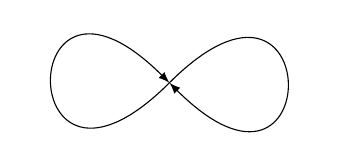
\begin{tikzpicture}
      \path[use as bounding box] (-1.8, -0.7) rectangle (1.8,0.7);
      \draw [-latex] (0, 0) .. controls (2, 2) and (2, -2) .. (0, 0);
      \draw [-latex] (0, 0) .. controls (-2, -2) and (-2, 2) .. (0, 0);
    \end{tikzpicture}
\end{center}
\end{ex}

\begin{ex}
Consider the line $\mathbb{R}$, and define the map $f:\mathbb{R}\rightarrow T^2=\mathbb{R^2}/\mathbb{Z}^2$ by $f(x)=\alpha x$, where $\alpha$ is some irrational number. Then this map gives an immersed submanifold of $T^2$, but is not an embedded submanifold, since $\mathbb{R}$ certainly does not have the subspace topology from $T^2$.
\end{ex}

Given the above definition, it seems rather difficult to construct submanifolds. For example, it is not immediately clear whether 
\[
S^n=\{\mathbf{x}\in\mathbb{R}^{n+1}:|\mathbf{x}|\leq1\}\subseteq\mathbb{R}^{n+1}
\]
is an embedded submanifolds, even though it feels like it should be.

More generally, if $M$, $N$ are manifolds, $F\in C^\infty(M,N)$ and $c\in N$, under what circumstances will $F^{-1}(c)$ be an embedded submanifold of $M$?

\begin{defn}
Let $F\in C^\infty(M,N)$ and $c\in N$. Let $S=F^{-1}(c)$. Then we say that $c$ is a \emph{regular value} if $\forall p\in S$, the map $DF|_p:T_pM\rightarrow T_cN$ is surjective.
\end{defn}

\begin{prop}
Let $F\in C^\infty(M,N)$ and let $c\in N$. Suppose $c$ is a regular value. Then $S=F^{-1}(c)$ is an embedded submanifold of dimension $\dim M-\dim N$.
\end{prop}

\begin{proof}
Let $n=\dim M$ and $m=\dim N$. For the map $DF$ to be surjective, we must have $n\geq m$.

Let $p\in S$, s.t. $F(p)=c$. We want to find a slice coord for $S$ near $p$. This problem is local, so by restricting to local coord charts, we may wlog assume $N=\mathbb{R}^m$, $M=\mathbb{R}^n$ and c=p=0.

Thus we have a smooth map $F:\mathbb{R}^n\rightarrow\mathbb{R}^m$ with surjective derivative at 0. This derivative is
\[
\left(\left.\frac{\partial F_j}{\partial x_i}\right|_0\right)_{i=1,...,n;j=1,...,m}\,,
\]
which by assumption has rank $m$. We re-order the $x_i$ so that the first $m$ columns are independent. Then the $m\times m$ matrix
\[
R=\left(\left.\frac{\partial F_j}{\partial x_i}\right|_0\right)_{i,j=1,...,m}
\]
is non-singular. Now consider the map
\[
\alpha(x_1,...,x_n)=(F_1,...,F_m,x_{m+1},...,x_n)\,.
\]
This gives
\[
D\alpha|_0=\begin{pmatrix}
R & *\\
0 & I
\end{pmatrix}\,,
\]
which is non-singular. By the inverse function theorem, $\alpha$ is a local diffeomorphism. So $\exists$ open $W\subseteq\mathbb{R}^n$ containing 0 s.t. $\alpha|_W:W\rightarrow \alpha(W)$ is smooth with smooth inverse.

Now since $\alpha$ is a smooth diffeomorphism, it is certainly a chart. Moreover by construction, the points in $S$ are exactly those whose image under $F$ have the first $m$ coords vanish. So $\alpha$ is a slice chart of $S$ in $\mathbb{R}^n$.
\end{proof}

\begin{ex}
We want to show that $S^n$ is a manifold. Let $F:\mathbb{R}^{n+1}\rightarrow\mathbb{R}$ be defined by
\[
F(x_0,...,x_n)=\sum x_i^2\,.
\]
Then $F^{-1}(1)=S^n$, and
\[
DF|_p=2(x_0,...,x_n)\neq0
\]
when $p\in S^n$. So $S^n$ is a manifold.
\end{ex}

\begin{ex}
Consider the orthogonal group. Let $M_n\simeq\mathbb{R}^{n^2}$ be space of all $n\times n $ matrices with the obvious smooth structure. We define
\[
N=\{A\in M_n: A^T=A\}
\]
Since this is a linear subspace, it is also a manifold. Define
\begin{align*}
    F:M_n&\rightarrow N\\
    A&\mapsto AA^T\,.
\end{align*}
Then we have
\[
O(n)=F^{-1}(I)=\{A:AA^T=I\}\,.
\]
We compute the derivative by looking at
\[
F(A+H)=(A+H)(A+H)^T=AA^T+HA^T+AH^T+HH^T\,.
\]
Then
\[
DF|_A(H)=HA^T+AH^T\,.
\]
So if $A\in O(n)$, then
\[
DF|_A(HA)=HAA^T+AA^TH^T=H+H^T
\]
for any $H$. Since every symmetric matrix is of the form $H+H^T$, we know that $DF|_A:T_AM_n\rightarrow T_{F(A)}N$ is surjective. So $O(n)$ is a manifold.
\end{ex}

\section{Vector fields}
\subsection{The tangent bundle}

Recall that we had the notion of a tangent vector. If we have a curve $\gamma:I\rightarrow M$, then we want to think of the derivative $\dot{\gamma}$ ``varying smoothly" with time. However we cannot do that yet, since for different $t$, the value of $\dot{\gamma}$ lies in different vector spaces, and we do not have a way of comparing them.

More generally, given a ``vector field" $f:p\mapsto v_p\in T_pM$ for each $p\in M$, we want to be able to know if it is a smooth function.

One way to solve this is to pick local coords $x_1,...,x_n$ on $U\subseteq M$. We can then write
\[
v_p=\sum_i\alpha_i(p)\left.\frac{\partial}{\partial x_i}\right|_p\,.
\]
Since $\alpha_i(p)\in\mathbb{R}$, we can say that $v_p$ varies smoothly if the functions $\alpha_i(p)$ are smooth. We then proceed to check that this does not depend on coords etc.

There is a more direct approach. We simply turn
\[
TM=\bigcup_{p\in M}T_pM
\]
into a manifold. Then there is a natural map $\pi:TM\rightarrow M$ sending $v_p\in T_pM$ to $p$ for each $p\in M$, which is smooth. We can then define smoothness of $f$ using the usual notion of smoothness of maps between manifolds.

\begin{defn}[Vector field]
A \emph{vector field} on some $U\subseteq M$ is a smooth map $X:U\rightarrow TM$ s.t. $\forall p\in U$, we have
\[
X(p)\in T_pM\,.
\]
In other words, we have $\pi\circ X=\text{id}$.
\end{defn}

\begin{defn}[$\Vect(U)$]
Let $\Vect(U)$ denote the set of all vector fields on $U$. Let $X,Y\in\Vect(U)$, and $f\in C^\infty(U)$. Then we can define
\[
(X+Y)(p)=X(p)+Y(p),\qquad (fX)(p)=f(p)X(p)\,.
\]
Then we have $X+Y, fX\in\Vect(U)$. So $\Vect(U)$ is a $C^\infty(U)$ module.
\end{defn}

Moreover if $V\subseteq U\subseteq M$ and $X\in\Vect(U)$, then $X|_V\in\Vect(V)$. Conversely if $\{V_i\}$ is cover of $U$ and $X_i\in\Vect(V_i)$ are s.t. they agree on intersections, then they patch together to give an element of $\Vect(U)$. So we say that $\Vect$ is a \emph{sheaf of} $C^\infty(M)$ \emph{modules}.

\begin{defn}[Tangent bundle]
Let $M$ be a manifold, and
\[
TM=\bigcup_{p\in M}T_pM\,.
\]
There is a natural projection map $\pi:TM\rightarrow M$ sending $v_p\in T_pM$ to $p$.

Let $x_1,...,x_n$ be coords on a chart $(U,\varphi)$. Then for any $p\in U$ and $v_p\in T_pM$, there are some $\alpha_1,...,\alpha_n\in\mathbb{R}$ s.t.
\[
v_p=\sum_{i=1}^n\alpha_i\left.\frac{\partial}{\partial x_i}\right|_p\,.
\]
This gives a bijection
\begin{align*}
    \pi^{-1}(U)&\rightarrow\varphi(U)\times\mathbb{R}^n\\
    v_p&\mapsto(x_1(p),...,x_n(p),\alpha_1,...,\alpha_n)\,.
\end{align*}
These charts make $TM$ into a manifold of dimension $2\dim M$, called the \emph{tangent bundle of} $M$. 
\end{defn}

\begin{lem}
The charts actually make $TM$ into a manifold.
\end{lem}

\begin{proof}
If $(V,\xi)$ is another chart on $M$ with coords $y_1,...,x_n$, then 
\[
\left.\frac{\partial}{\partial x_i}\right|_p=\sum_{j=1}^n\frac{\partial y_j}{\partial x_i}(p)\left.\frac{\partial}{\partial y_j}\right|_p\,.
\]
So we have $\tilde{\xi}\circ\tilde{\varphi}^{-1}:\varphi(U\cap V)\times\mathbb{R}^n\rightarrow\xi(U\cap V)\times\mathbb{R}^n$ given by
\[
\tilde{\xi}\circ\tilde{\varphi}^{-1}(x_1,...,x_n,\alpha_1,...,\alpha_n)=\left(y_1,...,y_n,\sum_{i=1}^n\alpha_i\frac{\partial y_1}{\partial x_i},...,\sum_{i=1}^n\alpha_i\frac{\partial y_n}{\partial x_i}\right)\,,
\]
and is smooth (and in fact fiberwise linear).

It is then easy to check that $TM$ is Hausdorff and second countable as $M$ is.
\end{proof}

\begin{rmks}
\leavevmode
\begin{enumerate}
    \item The projection map $\pi:TM\rightarrow M$ is smooth.
    \item If $U\subseteq M$ open, recall that
    \[
    \Vect(U)=\{\text{smooth }X:U\rightarrow TM|X(p)\in T_pM\;\forall p\in U\}\,.
    \]
    Write $X_p$ for $X(p)$. Now suppose further that $U$ is a coord chart. Then we can write any function $X:U\rightarrow TM$ s.t. $X_p\in T_pM$ (uniquely) as
    \[
    X_p=\sum_{i=1}^n\alpha_i(p)\left.\frac{\partial}{\partial x_i}\right|_p\,.
    \]
    Then $X$ is smooth iff all $\alpha_i$ are smooth.
    \item If $F\in C^\infty(M,N)$, then $DF:TM\rightarrow TN$ given by $DF(v_p)=DF|_p(v_p)$ is smooth. This allows us to talk about higher derivatives by simply taking further derivatives of the derivative map.
    \item If $F\in C^\infty(M,N)$ and $X$ vector field on $M$, then we \emph{cannot} obtain a vector field on $N$ by $DF(X)$, since $F$ might not be injective. If $F(p_1)=F(p_2)$, we need not have $DF(X(p_1))=DF(X(p_2))$.
\end{enumerate}
\end{rmks}

There is a weaker notion of being $F$-related.
\begin{defn}[F-related]
Let $M,N$ be manifolds, and $X\in\Vect(M)$, $Y\in\Vect(N)$ and $F\in C^\infty(M,N)$. Then they are $F$\emph{-related} if
\[
Y_q=DF|_p(X_p)
\]
for all $p\in M$ and $F(p)=q$. In other words, if the following diagram commutes
\[
\begin{tikzcd}
TM\arrow{r}{DF}&TN\\
M\arrow{u}{X}\arrow{r}{F}&N\arrow{u}{Y}
\end{tikzcd}\,,
\]
then we say that $X$, $Y$ are $F$-related.
\end{defn}

We now want to know what $\Vect(M)$ might look like. Recall that a vector is defined to be a derivation, so perhaps a vector field is also a derivation of some sort.

\begin{defn}[$\Der(C^\infty(M))$]
Let $\Der(C^\infty(M))$ be set of all $\mathbb{R}$-linear maps $\mathcal{X}:C^\infty(M)\rightarrow C^\infty(M)$ that satisfy
\[
\mathcal{X}(fg)=f\mathcal{X}(g)+\mathcal{X}(f)g\,.
\]
This is an $\mathbb{R}$-vector space, and in fact a $C^\infty(M)$ module.
\end{defn}

Given $X\in\Vect(M)$, we get a derivation $\mathcal{X}\in\Der(C^\infty(M))$ by setting
\[
\mathcal{X}(f)(p)=X_p(f)\,.
\]
It is possible to show that $\mathcal{X}(f)$ is smooth and satisfies the Leibniz rule. Similar to the case of vectors, we want to show that all derivations come from vector fields.

\begin{lem}
The map $X\mapsto\mathcal{X}$ is an $\mathbb{R}$-linear isomorphism
\[
\Gamma:\Vect(M)\rightarrow\Der(C^\infty(M))\,.
\]
\end{lem}

\begin{proof}
Suppose that $\alpha$ is a derivation. If $p\in M$, define
\[
X_p(f)=\alpha(f)(p)
\]
for all $f\in C^\infty(M)$. This is a linear map, with
\[
X_p(fg)=\alpha(fg)(p)=(f\alpha(g)+g\alpha(f))(p)=f(p)X_p(g)+g(p)X_p(f)\,.
\]
So $X_p\in T_pM$. We now check that the map $M\rightarrow TM$ sending $p\mapsto X_p$ is smooth. Locally on $M$, we have coords $x_1,...,x_n$, and we can write
\[
X_p=\sum_{i=1}^n\alpha_i(p)\left.\frac{\partial}{\partial x_i}\right|_p\,,
\]
where $\alpha_i:U\rightarrow\mathbb{R}$. Now pick bump function $\varphi$ that is identically 1 near $p$, with $\text{supp}\,\varphi\subseteq U$. Consider the function $\varphi x_j\in C^\infty(M)$. We can then consider
\[
\alpha(\varphi x_j)(p)=X_p(\varphi x_j)\,.
\]
As $\varphi x_j$ is just $x_j$ near $p$, by properties of derivations we know this is equal to $\alpha_j$. So we have $\alpha(\varphi x_j)=\alpha_j$, i.e. $\alpha_j$ is smooth. So $X_p$ is smooth.
\end{proof}

From now on we confuse $X$ and $\mathcal{X}$, i.e. we think of any $X\in\Vect(M)$ as a derivation of $C^\infty(M)$.

Note that the product of two vector fields (i.e. the composition of derivations) is not a vector field. This is since
\begin{align*}
    XY(fg)&=X(Y(fg))\\
    &=X(fY(g)+gY(f))\\
    &=X(f)Y(g)+fXY(g)+X(g)Y(f)+gXY(f)
\end{align*}
gives cross terms $X(f)Y(g)$. Instead, we have that $XY-YX$ is a derivation.

\begin{defn}[Lie bracket]
If $X,Y\in\Vect(M)$, then the \emph{Lie bracket} $[X,Y]$ is (the vector field corresponding to) the derivation $XY-YX\in\Vect(M)$.
\end{defn}

So $\Vect(M)$ becomes a \emph{Lie algebra}.

\subsection{Flows}
Imagine that a manifold represents all space, with a vector field specifying the velocity of a particle at that point. Then if we placed a particle at that point, it should move according to the velocity specified. Thus the vector field generates a \emph{flow} of the particle. These trajectories are known as \emph{integral curves}.

\begin{defn}[Integral curve]
Let $X\in\Vect(M)$. An \emph{integral curve} of $X$ is a smooth $\gamma:I\rightarrow M$ s.t. $I$ is an open interval in $\mathbb{R}$ and
\[
\dot{\gamma}(t)=X_{\gamma(t)}\,.
\]
\end{defn}

\begin{ex}
Take $M=\mathbb{R}^2$, and let
\[
X=x\frac{\partial}{\partial y}-y\frac{\partial}{\partial x}\,.
\]
This field looks like
\begin{figure}[h]
    \centering
    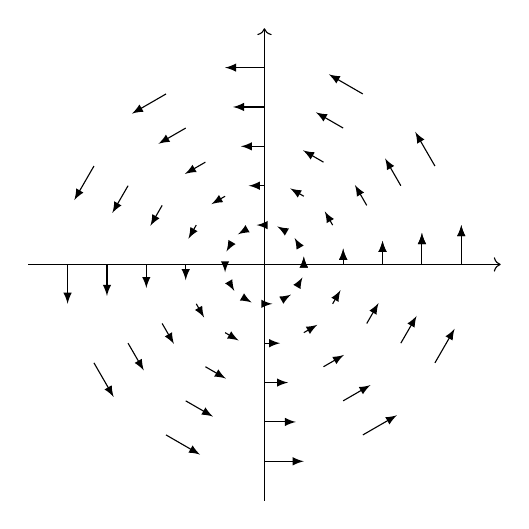
\begin{tikzpicture}
        \draw [->] (-3, 0) -- (3, 0);
        \draw [->] (0, -3) -- (0, 3);

        \foreach \t in {0,30,60,90,120,150,180,210,240,270,300,330,360} {
            \begin{scope}[rotate=\t]
                \draw [-latex] (2.5, 0) -- +(0, 0.5);
                \draw [-latex] (2, 0) -- +(0, 0.4);
                \draw [-latex] (1.5, 0) -- +(0, 0.3);
                \draw [-latex] (1, 0) -- +(0, 0.2);
                \draw [-latex] (0.5, 0) -- +(0, 0.1);
            \end{scope}
        }
    \end{tikzpicture}
\end{figure}

so we would expect the integral curves to be circles. Indeed, suppose $\gamma:I\rightarrow\mathbb{R}^2$ is an integral curve. Writing $\gamma=(\gamma_1,\gamma_2)$, the definition then requires
\[
\gamma_1'(t)\frac{\partial}{\partial x}+\gamma_2'(t)\frac{\partial}{\partial y}=\gamma_1(t)\frac{\partial}{\partial y}=\gamma_2(t)\frac{\partial}{\partial x}\,.
\]
So we have
\begin{align*}
    \gamma_1'(t)&=-\gamma_2(t)\,,\\
    \gamma_2'(t)&=\gamma_1(t)\,.
\end{align*}
This amounts to just solving an ordinary differential equation. For example if our starting point is $p=(1,0)$, we have
\[
\gamma_1(t)=\cos t\,,\qquad\gamma_2(t)=\sin t\,.
\]
\end{ex}

So to find an integral curve, we simply need to solve an ordinary differential equation, and since all ODEs have smooth and unique solutions, they have all the nice properties we can hope for. But sometimes funny things can happen.

\begin{ex}
Take $M=\mathbb{R}$, and 
\[
X=x^2\frac{d}{dx}\,.
\]
Then if $\gamma$ is an integral curve, it must satisfy
\[
\gamma'(t)=\gamma(t)^2\,.
\]
This has a solution of the form
\[
\gamma(t)=\frac{1}{C-t}
\]
where $C$ is a constant. For example if we want $\gamma(0)=\frac{1}{2}$, then we have
\[
\gamma(t)=\frac{1}{2-t}\,.
\]
This solution is defined for only $t<2$, so we can only have $I=(-\infty,2)$ at best.
\end{ex}

We now prove that integral curves always exist. To do so, we first need some theorems from ODE theory.

\begin{thm}[Fundamental theorem of ODEs]
Let $U\subseteq\mathbb{R}^n$ be open and $\alpha:U\rightarrow\mathbb{R}^n$ smooth. Pick $t_0\in\mathbb{R}$\,.

Consider the ODE
\begin{align*}
    \dot{\gamma}_i(t)&=\alpha_i(\gamma(t))\\
    \gamma_i(t_0)&=c_i\,,
\end{align*}
where $\mathbf{c}=(c_1,...,c_n)\in\mathbb{R}^n$. Then there exists an open interval $I$ containing $t_0$ and open $U_0\subseteq U$ s.t. for every $\mathbf{c}\in U_0$, there is a smooth solution $\gamma_\mathbf{c}:I\rightarrow U$ satisfying the ODE. Moreover, any two solutions agree on a common domain, and the function $\Theta:I\times U_0\rightarrow U$ defined by $\Theta(t,\mathbf{c})=\gamma_\mathbf{c}(t)$ is smooth (in both variables).
\end{thm}

\begin{thm}[Existence and uniquness of integral curves]
Let $X\in\Vect(M)$ and $p\in M$. Then there exists some open interval $I\subseteq\mathbb{R}$ with $0\in I$ and integral curve $\gamma:I\rightarrow M$ for $X$ s.t. $\gamma(0)=p$. Moreover if $\tilde{\gamma}:\tilde{I}\rightarrow M$ is another integral curve for $X$, and $\tilde{\gamma}(0)=p$, then $\tilde{\gamma}=\gamma$ on $I\cap\tilde{I}$.
\end{thm}

\begin{proof}
Pick local coords for $M$ centered at $p$ in an open nhood $U$. Locally we write
\[
X=\sum_{i=1}^n\alpha_i\frac{\partial}{\partial x_i}\,,
\]
where $\alpha_i\in C^\infty(U)$. We want to find $\gamma=(\gamma_1,...,\gamma_n):I\rightarrow U$ s.t.
\[
\sum_{i=1}^n\gamma_i'(t)\left.\frac{\partial}{\partial x_i}\right|_{\gamma(t)}=\sum_{i=1}^n\alpha_i(\gamma(t))\left.\frac{\partial}{\partial x_i}\right|_{\gamma(t)}\,,\qquad\gamma_i(0)=0\,.
\]
Since the $\frac{\partial}{\partial x_i}$ form a basis, this is equivalent to saying
\[
\gamma_i(t)=\alpha_i(\gamma(t))\,,\qquad\gamma_i(0)=0
\]
for all $i$ and $t\in I$.

By general theory of ODEs, there is an interval $I$ and solution $\gamma$, with any two solutions agreeing on their common domain.

For uniqueness, first note that we know that there is a unique integral curve lying in this particular chart. So suppose $\gamma:I\rightarrow M$, $\tilde{\gamma}:\tilde{I}\rightarrow M$ are both integral curves passing through the same point, i.e. $\gamma(0)=\tilde{\gamma}(0)=p$. Let
\[
J=\{t\in I\cap \tilde{I}:\gamma(t)=\tilde{\gamma}(t)\}\,.
\]
This is non-empty since $0\in J$, and $J$ is closed since $\gamma$, $\tilde{\gamma}$ continuous. So let $t_0\in J$, and consider $q=\gamma(t_0)$. Then $\gamma$, $\tilde{\gamma}$ are integral curves of $X$ passing through $q$. By the first part, they agree on some neighbourhood of $t_0$. So $J$ is open. By connectedness, this means that $J=I\cap\tilde{I}$.
\end{proof}

\begin{defn}[Maximal integral curve]
Let $p\in M$, and $X\in\Vect(M)$. Let $I_p$ be union of all $I$ s.t. there is an integral curve $\gamma:I\rightarrow M$ with $\gamma(0)=p$. Then there exists a unique integral curve $\gamma:I_p\rightarrow M$ known as the \emph{maximal integral curve}.
\end{defn}

Note that $I_p$ does depend on the point.

\begin{ex}
Consider the vector field
\[
X=\frac{\partial}{\partial x}
\]
on $\mathbb{R}^2\setminus\{0\}$. Then for any point $p=(x,y)$, if $y\neq0$, we have $I_p=\mathbb{R}$, but if $y=0$ and $x<0$, then $I_p=(-\infty,-x)$. Similarly if $y=0$ and $x>0$, then $I_p=(-x,\infty)$.

\begin{figure}[h]
    \centering
    \begin{tikzpicture}
        \draw (-3, 3) rectangle (3, -3);
        \foreach \x in {-2.7, -1.7, -0.7, 0.3, 1.3, 2.3} {
            \foreach \y in {-2, -1, 0, 1, 2} {
            \draw [-latex] (\x, \y) -- +(0.4, 0);
            }
        }
        \draw circle [radius=0.1];
    \end{tikzpicture}
\end{figure}
\end{ex}

\begin{defn}[Complete vector field]
A vector field is \emph{complete} if $I_p=\mathbb{R}\;\forall p\in M$.
\end{defn}

Given a complete vector field, we can obtain a flow map as follows,

\begin{thm}
Let $M$ be manifold and $X$ complete vector field on $M$. Define $\Theta_t:\mathbb{R}\times M\rightarrow M$ by
\[
\Theta_t(p)=\gamma_p(t)\,,
\]
where $\gamma_p$ is the maximal integral curve of $X$ through $p$ with $\gamma(0)=p$. Then $\Theta$ is a function smooth in $p$ and $t$, and 
\[
\Theta_0=\text{id}\,,\qquad\Theta_t\circ\Theta_s=\Theta_{s+t}\,.
\]
\end{thm}

\begin{proof}
This follows from uniqueness of integral curves and smooth dependence on initial conditions of ODEs.
\end{proof}

In particular, since $\Theta_t\circ\Theta_{-t}=\Theta_0=\text{id}$, we know that
\[
\Theta^{-1}_t=\Theta_{-t}\,.
\]
So $\Theta$ is a diffeomorphism. Algebraically, if we write $\Diff(M)$ as the group of diffeomorphisms $M\rightarrow M$, then 
\begin{align*}
    \mathbb{R}&\rightarrow\Diff(M)\\
    t&\mapsto\Theta_t
\end{align*}
is a homomorphism of groups. We call this a \emph{one-parameter subgroup} of diffeomorphisms.

\begin{thm}
Let $M$ be manifold, $X\in\Vect(M)$. Define
\[
D=\{(t,p)\in\mathbb{R}\times M:t\in I_p\}\,.
\]
This is the set of all $(t,p)$ s.t. $\gamma_p(t)$ exists. Set
\[
\Theta_t(p)=\Theta(t,p)=\gamma_p(t)
\]
for all $(t,p)\in D$. Then
\begin{enumerate}
    \item $D$ is open and $\Theta: D\rightarrow M$ is smooth
    \item $\Theta(0,p)=p\;\forall p\in M$
    \item If $(t,p)\in D$ and $(t,\Theta(s,p))\in D$, then $(s+t,p)\in D$ and $\Theta(t,\Theta(s,p))=\Theta(t+s,p)$
    \item For any $t\in\mathbb{R}$, the set $M_t:\{p\in M:(t,p)\in D\}$ is open in $M$, and 
    \[
    \Theta_t:M_t\rightarrow M_{-t}
    \]
    is a diffeomorphism with inverse $\Theta_{-t}$.
\end{enumerate}
\end{thm}

So when the assumption of completeness is relaxed, we have to take care of the domains of definition. This rather troublesome, so in nice cases we can avoid these problems by using the following result.

\begin{prop}
Let $M$ be compact manifold. Then any $X\in\Vect(M)$ is complete.
\end{prop}

\begin{proof}
Recall that
\[
D=\{(t,p):\Theta_t(p)\text{ is defined}\}
\]
is open. So given $p\in M$, there is some open nhood $U\subseteq M$ of $p$ and an $\varepsilon>0$ s.t. $(-\varepsilon,\varepsilon)\times U\subseteq D$. By compactness, we can find finitely many such $U$ that cover $M$, and find small $\varepsilon$ s.t. $(-\varepsilon,\varepsilon)\times M\subseteq D$.

In other words, we know that $\Theta_t(p)$ exists and $p\in M$ and $|t|<\varepsilon$. Also we know that $\Theta_t\circ\Theta_s=\Theta_{t+s}$ whenever $|t|,|s|<\varepsilon$, and in particular $\Theta_{t+s}$ is defined. So $\Theta_{Nt}=(\Theta_t)^N$ is defined for all $N$ and $|t|<\varepsilon$, so $\Theta_t$ is defined for all $t$.
\end{proof}

\subsection{Lie derivative}

Given a function $f$ defined on all of $M$, we can calculate its derivative along a vector field $X$ at each point using $X(f)$. However this only works when $f$ is real-valued. For something more complicated, we can still differentiate things along $X$ using flows.

\begin{notn}
Let $F:M\rightarrow M$ be diffeo, and $g\in C^\infty(M)$. We write
\[
F^*g=g\circ F\in C^\infty(M)\,.
\]
\end{notn}

\begin{defn}[Lie derivative of a function]
Let $X$ be complete vector field, and $\Theta$ its flow. The \emph{Lie derivative} of $g$ along $X$ is
\[
\mathcal{L}_X(g)=\left.\frac{d}{dt}\right|_{t=0}\Theta^*_tg\,.
\]
This is defined pointwise, i.e. for all $p\in M$, we have
\[
\mathcal{L}_X(g)(p)=\left.\frac{d}{dt}\right|_{t=0}\Theta^*_t(g)(p)\,.
\]
\end{defn}

\begin{lem}
$\mathcal{L}_X(g)=X(g)$. In particular, $\mathcal{L}_X(g)\in C^\infty(M,\mathbb{R})$\,.
\end{lem}
\begin{proof}
\begin{align*}
    \mathcal{L}_X(g)(p)&=\left.\frac{d}{dt}\right|_{t=0}\Theta^*_t(g)(p)\\
    &=\left.\frac{d}{dt}\right|_{t=0}g(\Theta_t(p))\\
    &=dg|_(X(p))\\
    &=X(g)(p)\,.
\end{align*}
\end{proof}

\begin{notn}
Let $Y\in\Vect(M)$, and $F:M\rightarrow M$ be diffeo. Then $DF^{-1}|_{F(p)}:T_{F(p)}M\rightarrow T_p M$. So we can write
\[
F^*(Y)|_p=DF^{-1}|_{F(p)}(Y_{F(p)})\in T_pM\,.
\]
Then $F^*(Y)\in\Vect(M)$. If $g\in C^\infty(M)$, then 
\[
F^*(Y)|_p(g)=Y_{F(p)}(g\circ F^{-1})\,.
\]
Alternatively, we have 
\[
F^*(Y)|_p(g\circ F)=Y_{F(p)}(g)\,,
\]
or without the $p$'s, we have
\[
F^*(Y)(g\circ F)=(Y(g))\circ F\,.
\]
\end{notn}

\begin{defn}[Lie derivative of a vector field]
Let $X\in\Vect(M)$ be complete, and $Y\in\Vect(M)$ be vector field. Then the \emph{Lie derivative} is given pointwise by
\[
\mathcal{L}_X(Y)=\left.\frac{d}{dt}\right|_{t=0}\Theta^*_t(Y)\,.
\]
\end{defn}

\begin{lem}
$\mathcal{L}_XY=[X,Y]$.
\end{lem}

\begin{proof}
Let $g\in C^\infty(M,\mathbb{R})$. Then we have
\[
\Theta^*_t(Y)(g\circ\Theta_t)=Y(g)\circ\Theta_t\,.
\]
So consider
\[
\frac{\Theta^*_t(Y)(g)-Y(g)}{t}=\underbrace{\frac{\Theta^*_t(Y)(g)-\Theta^*_t(Y)(g\circ\Theta_t)}{t}}_{\alpha_t}+\underbrace{\frac{Y(g)\circ\Theta_t-Y(g)}{t}}_{\beta_t}\,.
\]
Now $\lim_{t\rightarrow0}\beta_t=\mathcal{L}_X(Y(g))=XY(g)$ by the previous lemma, and
\[
\lim_{t\rightarrow0}\alpha_t=\lim_{t\rightarrow0}(\Theta^*_t(Y))\left(\frac{g-g\circ\Theta_t}{t}\right)=Y(-\mathcal{L}_X(g))=-YX(g)\,.
\]
\end{proof}

\begin{cor}
Let $X,Y\in\Vect(M)$ and $f\in C^\infty(M,\mathbb{R})$. Then
\begin{itemize}
    \item $\mathcal{L}_X(fY)=\mathcal{L}_X(f)Y+f\mathcal{L}_XY=X(f)Y+f\mathcal{L}_XY$
    \item $\mathcal{L}_XY=-\mathcal{L}_YX$
    \item $\mathcal{L}_X[Y,Z]=[\mathcal{L}_XY,Z]+[Y,\mathcal{L}_XZ]$.
\end{itemize}
\end{cor}

\section{Vector bundles}
Recall that we had the tangent bundle of a manifold. This gives us a vector space at each point in space, namely the tangent space. In general, a vector bundle is a vector space attached to each point of our manifold (in a smoothly-varying way).

\subsection{Tensors}
A motivation for tensors come from the study of bilinear maps. This is a function that takes in two vectors and returns a number, and is linear in both variables. An example of a bilinear map is the inner product. The volume form, an object which tells us the volume of a parallelepiped spanned by two vectors, is also a bilinear map.

\begin{defn}[Bilinear map]
Let $U,V,W$ be vector spaces. We define $\Bilin(V\times W,U)$ to be the functions $\alpha:V\times W\rightarrow U$ that are bilinear, i.e.
\begin{align*}
    \alpha(\lambda_1v_1+\lambda_2v_2,w)&=\lambda_1\alpha(v_1,w)+\lambda_2\alpha(v_2,w)\\
    \alpha(v,\lambda_1w_1+\lambda_2w_2)&=\lambda_1\alpha(v,w_1)+\lambda_2\alpha(v,w_2)\,.
\end{align*}
\end{defn}

It is important to note that a bilinear map is not a linear map. This makes all our results from linear algebra useless, but thankfully we have tensors, which are a trick to turn the study of bilinear maps into linear maps (from a different space).

\begin{defn}[Tensor product]
A \emph{tensor product} of two vector spaces $V,W$ is a vector space $V\otimes W$ and a bilinear map $\pi:V\times W\rightarrow V\otimes W$ s.t. a bilinear map from $V\times W$ is ``the same as" a linear map from $V\otimes W$. More precisely, given any bilinear map $\alpha:V\times W\rightarrow U$, we can find a unique linear map $\tilde{\alpha}:V\otimes W\rightarrow U$ s.t. the following diagram commutes:
\[
\begin{tikzcd}
V\times W\arrow{d}{\pi}\arrow{dr}{\alpha}\\
V\otimes W\arrow[swap]{r}{\tilde{\alpha}}&U
\end{tikzcd}
\]
So we have 
\[
\Bilin(V\times W,U)\cong\text{Hom}(V\otimes W,U)\,.
\]
Given $v\in V$ and $w\in W$, we obtain $\pi(v,w)\in V\otimes W$, called the \emph{tensor product} of $v$ and $w$, written $v\otimes w$.
\end{defn}

\end{document}
